\subsection{Identyfikacja aktorów}
W aplikacji występują cztery rodzaje użytkowników, z których każdy posiada określone uprawnienia, które pozwalają na korzystanie z określonych funkcjonalności. Poniżej przedstawiono listę aktorów wraz z ich uprawnieniami.
\begin{itemize}
    \item \textbf{Gość:} Użytkownik niezalogowany w aplikacji. Posiada dostęp do przeglądania warsztatów oraz nagród. Może zalogować i zarejestrować się za pomocą konta Google.
    \item \textbf{Użytkownik:} Użytkownik zalogowany w aplikacji. Posiada wszystkie uprawnienia Gościa. Dodatkowo może zapisać się na warsztat ograniczony ilością miejsc, przeglądać swój profil oraz skanować kody QR.
    \item  \textbf{Wolontariusz:} Użytkownik zalogowany w aplikacji. Posiada możliwość potwierdzania obecności uczestników na warsztatach.
    \item \textbf{Administrator:} Użytkownik zalogowany w aplikacji. Pełni w aplikacji znaczącą funkcję. Do jego zadań należy tworzenie i edycja warsztatów, nagród oraz kodów QR. Dodatkowo może edytować dane użytkowników oraz nadawać im role.
    \item \textbf{Prowadzący:} Użytkownik zalogowany w aplikacji. Posiada wszystkie uprawnienia Gościa. Dodatkowo może prowadzić warsztaty.
\end{itemize}
\subsection{Wymagania funkcjonalne i niefunkcjonalne}
Nazwa aplikacji to \textbf{UBB Events App}. W poniższych podsekcjach przedstawiono wymagania funkcjonalne oraz niefunkcjonalne postawione przed tworzoną aplikacją.
\subsubsection{Wymagania funkcjonalne}
Wymagania te stanowią podstawę do stworzenia aplikacji. Są to funkcjonalności, które muszą zostać zaimplementowane, aby aplikacja spełniała swoje zadanie. Poniżej przedstawiono listę wymagań funkcjonalnych aplikacji:
\begin{itemize}
    \item Rejestracja użytkownika za pomocą konta Google
    \item Logowanie użytkownika za pomocą konta Google
    \item Zapis danych użytkownika w bazie danych
    \item Przeglądanie dostępnych warsztatów
    \item Przeglądanie dostępnych nagród
    \item Zapis na warsztat ograniczony ilością miejsc
    \item Skanowanie kodu QR
    \item Wyświetlanie informacji o profilu użytkownika
    \item Losowanie nagród na podstawie punktów zdobytych przez użytkownika
    \item Tworzenie i edycja warsztatów przez administratora    
    \item Tworzenie i edycja nagród przez administratora
    \item Tworzenie i edycja kodów QR przez administratora
    \item Potwierdzanie obecności uczestnika na warsztatach przez administratora bądź wolontariusza
    \item Edycja danych użytkownika przez administratora
    \item Nadawanie ról użytkownikom przez administratora
\end{itemize}
\subsubsection{Wymagania niefunkcjonalne}
Wymagania niefunkcjonalne definiują dodatkowe cechy, które nie są zasadnicze dla podstawowego działania aplikacji, ale istotnie wpływają na jej jakość. Poniżej znajduje się lista takich wymagań dotyczących aplikacji:
\begin{itemize}
    \item Poprawne działanie aplikacji mobilnej na urządzeniach z systemem Android w wersji 5.0 lub nowszej
    \item Poprawne działanie aplikacji internetowej na przeglądarkach Google Chrome, Mozilla Firefox, Microsoft Edge, Safari
    \item Skalowalność aplikacji na różnych rozdzielczościach ekranu
\end{itemize}
\subsection{Encje bazy danych}
Do przechowywania danych jak już wcześniej wspomniano wykorzystano bazę PostgreSQL. Poniżej przedstawiono diagram encji bazy danych (\autoref{db}).
\begin{figure} [H]
    \begin{center}
    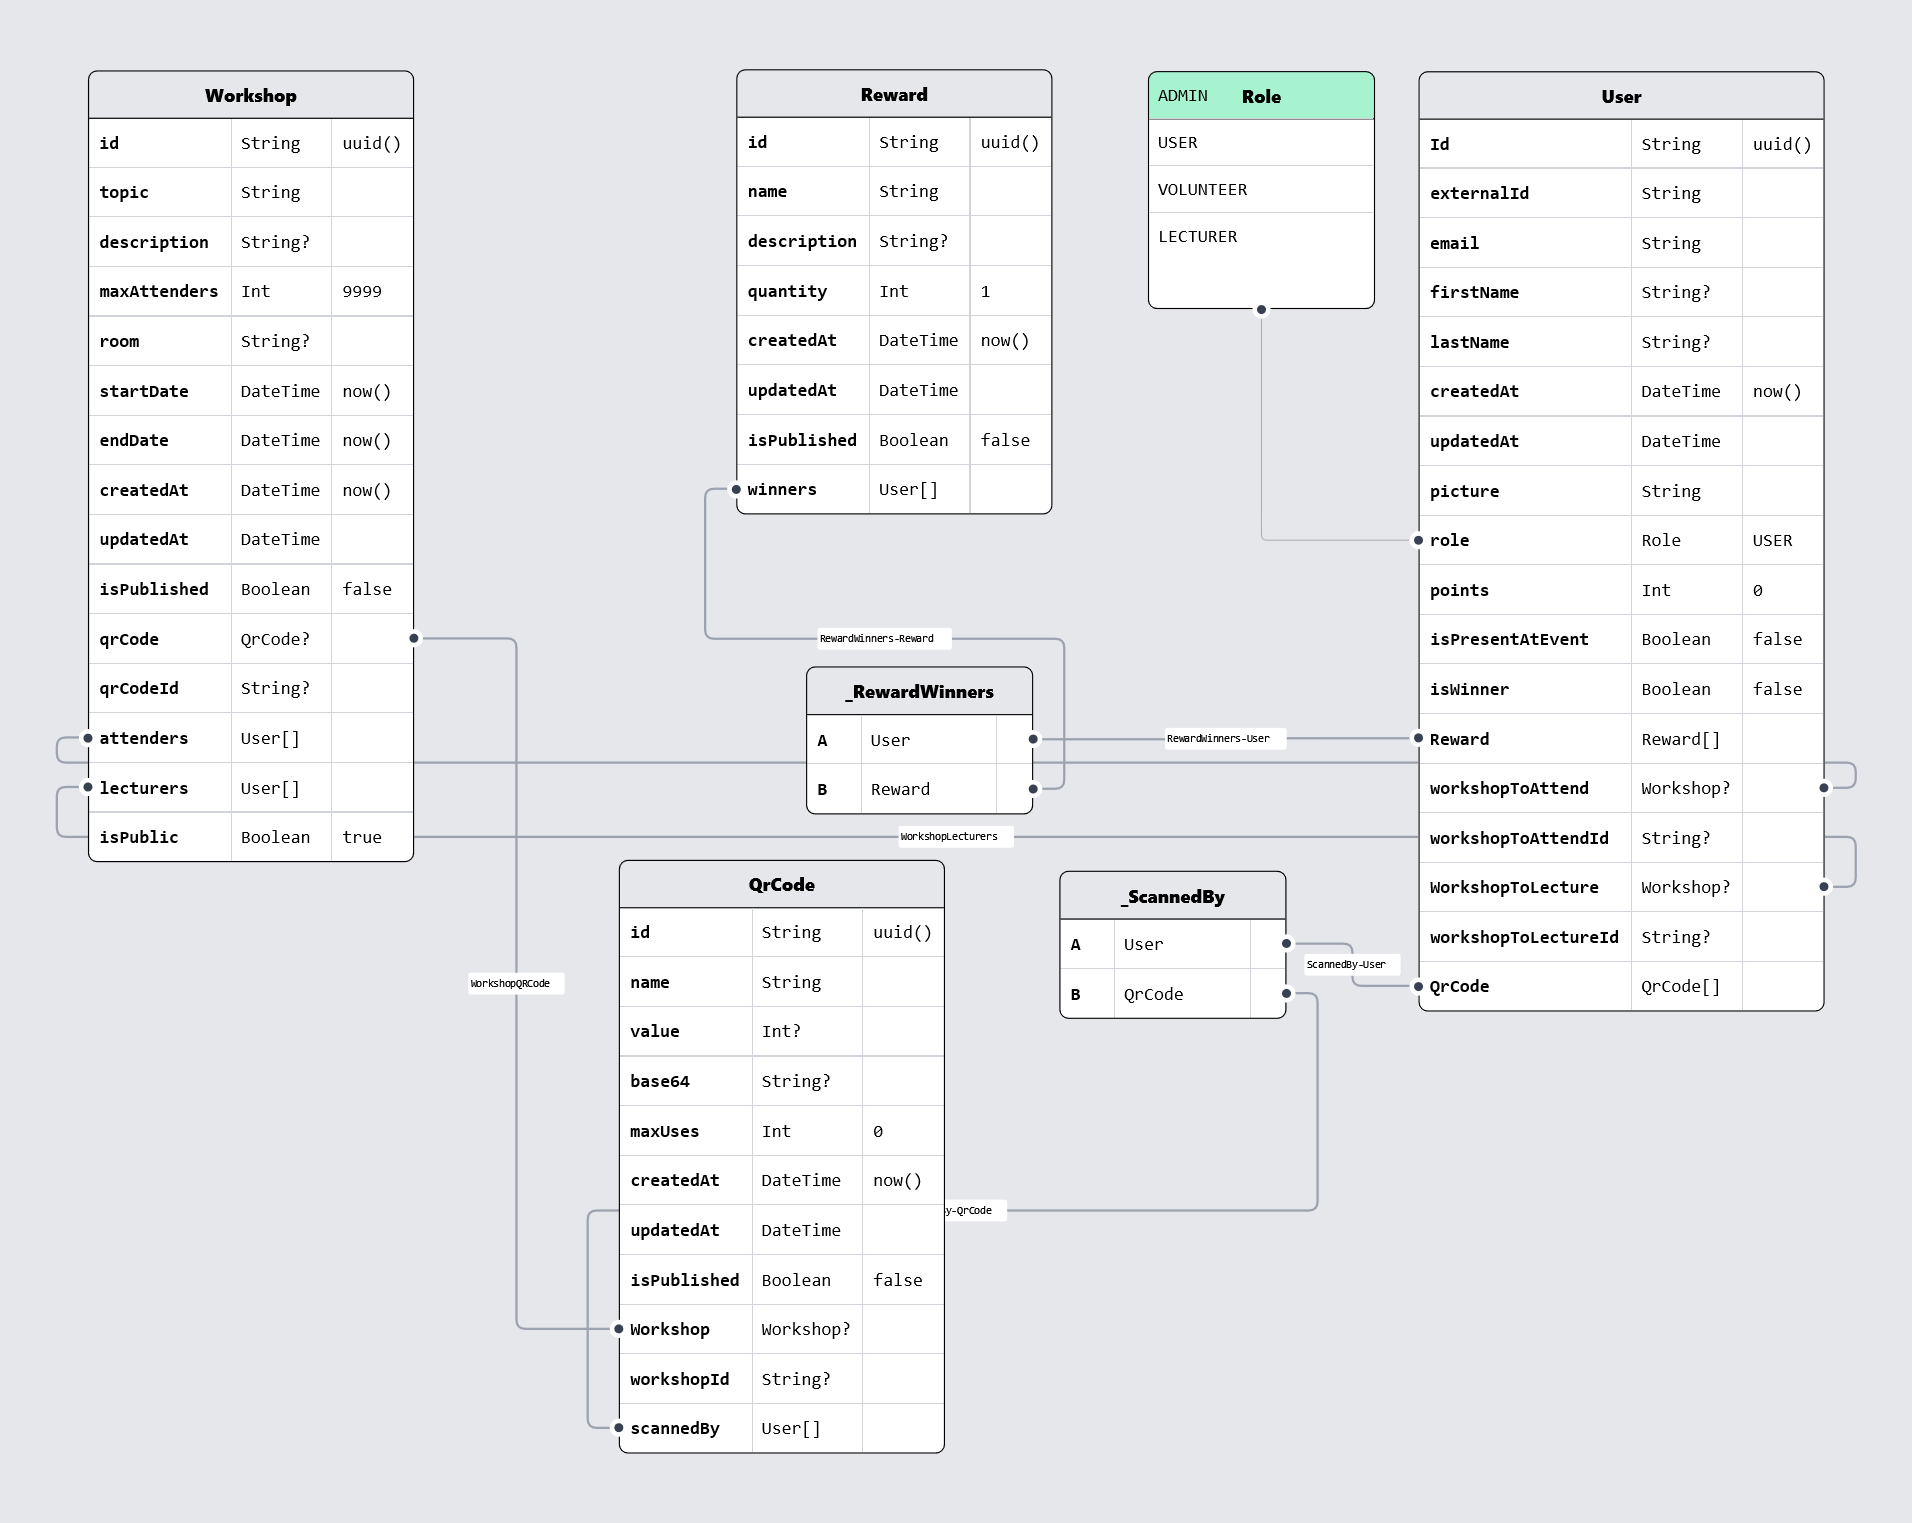
\includegraphics[scale=0.23]{imgs/database.png}
    \end{center}
    \caption{Diagram związków encji bazy danych}
    \label{db}
    \end{figure}
\noindent W bazie danych znajdują się cztery główne tabele:
\begin{itemize}
    \item \textbf{Użytkownicy} - przechowuje dane o użytkownikach aplikacji
    \item \textbf{Warsztaty} - przechowuje dane o  odbywających się warsztatach
    \item \textbf{Nagrody} - przechowuje dane o nagrodach możliwych do wygrania podczas warsztatów
    \item \textbf{Kody QR} - przechowuje dane o kodach QR mających wartość punktową
\end{itemize}

\subsubsection{Użytkownicy}
\noindent Użytkownicy to główna encja bazy danych.
\begin{itemize}
    \item \textbf{Id} - Główny klucz identyfikujący użytkownika
    \item \textbf{externalId} - Identyfikator użytkownika w systemie autoryzacji Clerk
    \item \textbf{email} - Adres email użytkownika
    \item \textbf{firstName} - Imię użytkownika
    \item \textbf{lastName} - Nazwisko użytkownika
    \item \textbf{createdAt} - Data utworzenia użytkownika
    \item \textbf{updatedAt} - Data ostatniej aktualizacji użytkownika
    \item \textbf{picture} - Adres URL do zdjęcia użytkownika
    \item \textbf{role} - Rola użytkownika w systemie (administrator, uczestnik, wolontariusz i prowadzący)
    \item \textbf{points} - Liczba zdobytych punktów przez użytkownika
    \item \textbf{isPresentAtEvent} - Zmienna logiczna określająca czy użytkownik jest obecny na wydarzeniu
    \item \textbf{isWinner} - Zmienna logiczna określająca czy użytkownik jest zwycięzcą jakiejkolwiek nagrody
    \item  \textbf{Reward} - Relacja wiele-do wielu z tabelą Nagrody. Przechowuje nagrody które użytkownik wygrał
    \item  \textbf{WorkshopToAttend} - Opcjonalna relacja z Warsztatem. Dla użytkownika który zapisał się na limitowany warsztat
    \item  \textbf{WorkshopToLecture} - Opcjonalna relacja z Warsztatem. Dla użytkownika któremu przypisano prowadzenie warsztatu
    \item  \textbf{QRCode} - Relacja wiele-do-wielu z tabelą Kody QR. Przechowuje zeskanowane kody QR przez użytkownika
\end{itemize}
\subsubsection{Warsztaty}
\noindent W tej encji przechowywane są dane o warsztatach odbywających się podczas wydarzenia.
\begin{itemize}
    \item \textbf{Id} - Główny klucz identyfikujący warsztat
    \item \textbf{topic} - Temat warsztatu
    \item \textbf{description} - Opcjonalny opis tego, co będzie się działo podczas warsztatu
    \item \textbf{MaxAttenders} - Maksymalna liczba uczestników warsztatu
    \item \textbf{room} - Sala w której odbywa się warsztat
    \item \textbf{startDate} - Data i godzina rozpoczęcia warsztatu
    \item  \textbf{endDate} - Data i godzina zakończenia warsztatu
    \item  \textbf{createdAt} - Data utworzenia warsztatu
    \item  \textbf{updatedAt} - Data ostatniej aktualizacji warsztatu
    \item  \textbf{isPublished} - Zmienna logiczna określająca czy warsztat jest upubliczniony
    \item   \textbf{QRCode} - Opcjonalna relacja jeden-do-jednego z tabelą Kody QR. Przechowuje kod QR dla warsztatu
    \item  \textbf{Lecturers} - Relacja jeden-do-wielu z tabelą Użytkownicy. Przechowuje prowadzących warsztat
    \item \textbf{Attenders} - Relacja jeden-do-wielu z tabelą Użytkownicy. Przechowuje uczestników
\end{itemize}
\subsubsection{Nagrody}
\noindent W tej encji przechowywane są dane o nagrodach możliwych do wygrani podczas wydarzenia. Losowane na podstawie punktów zebranych przez użytkowników.
\begin{itemize}
    \item \textbf{Id} - Główny klucz identyfikujący nagrodę
    \item \textbf{name} - Nazwa nagrody
    \item \textbf{description} - Opcjonalny opis nagrody
    \item \textbf{quantity} - Liczba sztuk poszczególnej nagrody
    \item \textbf{createdAt} - Data utworzenia nagrody
    \item \textbf{updatedAt} - Data ostatniej aktualizacji nagrody
    \item \textbf{isPublished} - Zmienna logiczna określająca czy nagroda jest upubliczniona
    \item \textbf{Winners} - Relacja wiele-do-wielu z tabelą Użytkownicy. Przechowuje użytkowników którzy wygrali nagrodę
    \end{itemize}
\subsubsection{Kody QR}
\noindent W tej encji przechowywane są dane o kodach QR mających wartość punktową.
\begin{itemize}
    \item \textbf{Id} - Główny klucz identyfikujący kod QR
    \item \textbf{name} - nazwa kodu QR
    \item  \textbf{value} - wartość punktowa kodu QR
    \item  \textbf{base64} - kod QR w formacie base64
    \item \textbf{createdAt} - Data utworzenia kodu QR
    \item \textbf{updatedAt} - Data ostatniej aktualizacji kodu QR
    \item \textbf{isPublished} - Zmienna logiczna określająca czy kod QR jest upubliczniony
    \item \textbf{Workshop} - Opcjonalna relacja jeden-do-jednego z tabelą Warsztaty. Przechowuje warsztat dla którego kod QR jest przeznaczony
    \item \textbf{scannedBy} - Relacja wiele-do-wielu z tabelą Użytkownicy. Przechowuje użytkowników którzy zeskanowali kod QR
    \end{itemize}
\subsection{Diagram przypadków użycia}
\input{sections/chapters/realization/przypadki.tex}
\subsection{Scenariusze przypadków użycia}
\subsection{Architektura aplikacji}
